% ------------------- IMPORTS -------------------
\documentclass[letterpaper,12pt]{article}
\usepackage{tabularx} % extra features for tabular environment
\usepackage{amsmath}  % improve maths presentation
\usepackage{amssymb} % maths symbols
\usepackage{graphicx} % takes care of graphic including machinery
\usepackage[margin=0.95in,letterpaper]{geometry} % decreases margins
\usepackage{cite} % takes care of citations
\usepackage[titletoc,title]{appendix} % takes care of appendices
\usepackage{listings} % code representation
\usepackage{pdflscape}
\usepackage{csquotes} % for quoting existing work
\usepackage{color} % defines colours for code listings
\usepackage{comment} % allows for block of comments
\usepackage{gensymb} % degree symbol
\usepackage[table,xcdraw]{xcolor} % table colouring
\usepackage[cc]{titlepic}  % allows a pic to be included in the title page
\usepackage[final]{hyperref} % adds hyper links inside the generated pdf file
\usepackage{pdfpages} % include pdfs

% ------------------- CODING STYLE -------------------
\definecolor{codegreen}{rgb}{0,0.6,0}
\definecolor{codegray}{rgb}{0.5,0.5,0.5}
\definecolor{backcolour}{rgb}{0.95,0.95,0.92}
\lstdefinestyle{mystyle}{
    backgroundcolor=\color{backcolour},   
    commentstyle=\color{codegreen},
    keywordstyle=\color{blue},
    numberstyle=\tiny\color{codegray},
    basicstyle=\footnotesize,
    breakatwhitespace=false,         
    breaklines=true,                 
    captionpos=b,                    
    keepspaces=true,                 
    numbersep=5pt,                  
    showspaces=false,                
    showstringspaces=false,
    showtabs=false,                  
    tabsize=4
}
\lstset{style=mystyle}

% ------------------- HEADINGS -------------------

\begin{document}

\title{
    Breast Cancer Detection in Mammograms using Deep Learning Techniques\\
    \vspace*{1cm}
    \begin{Large}
    Plan \& Context Survey\\
    \end{Large}
    \vspace*{1cm}
    \begin{large}
    University of St Andrews - School of Computer Science\\
    \end{large}
    \begin{large}
    Supervisor: Dr David Harris-Birtill
    \end{large}
    \vspace*{0.5cm}
}
\titlepic{
\includegraphics[width=0.35\linewidth]{figures/st-andrews-logo.jpeg}}
\author{Adam Jaamour} % Student ID: 150014151
\date{15th June, 2020}
\maketitle
\newpage

% ------------------- Thesis Outline --------------------

\section{Thesis Outline}
\label{sec:thesis-outline}

\paragraph{Introduction}
Sets the tone for the entire dissertation by presenting the subject and the problem being tackled, while also laying out the plan for the rest of the report. Subsections include the motivation \& problem description and the project aims.

\paragraph{Context Survey}
Explores the literature surrounding breast cancer detection using deep learning techniques, including state of the art techniques recently used, by covering the background of both deep learning techniques and their applications to the problem of breast cancer detection. See Section~\ref{sec:draft-context-survey} for this part's subsections.

\paragraph{Requirements}
Establishes and prioritises the functional and non-functional properties of the code.

\paragraph{Ethics}
Considers the ethical issues considered for this project.

\paragraph{Design}
Details the general structure of the system, offering an analysis of different parts of the deep learning pipeline without going into technical code-related or mathematics-related details. For example, this includes the choice of input method, data pre-processing steps, output format and programming languages and libraries.

\paragraph{Implementation}
Covers the specifics followed when implementing the deep learning pipeline, explaining the mathematical and software-related reasoning behind each decision (this will include equations and code snippets). Additionally, covers any testing done to validate that the system works as expected.

\paragraph{Evaluation}
Compare the final results with the basic pipeline’s results developed in common, the final results achieved by the two other group members and the results from papers researching breast cancer detection identified in the context survey.

\paragraph{Conclusions}
This sections will summarise the project as a whole, from the initial objective to the results obtained. Further discussions will be included to objectively assess what could have improved, as well as any potential future work.


% ------------------- Dissertation Time Plan --------------------

\section{Dissertation Time Plan}
\label{sec:time-plan}

Figure~\ref{fig:gantt_chart} showcases the estimated timeline for this dissertation, separating activities into four parts corresponding to the four main objectives established in the DOER document. These main activities are broken down into subactivities. Milestones are included in the Gantt chart as well. The chart was created using GanttProject\footnote{GanttProject: \url{https://www.ganttproject.biz/}}.

\begin{figure}[h]
\centerline{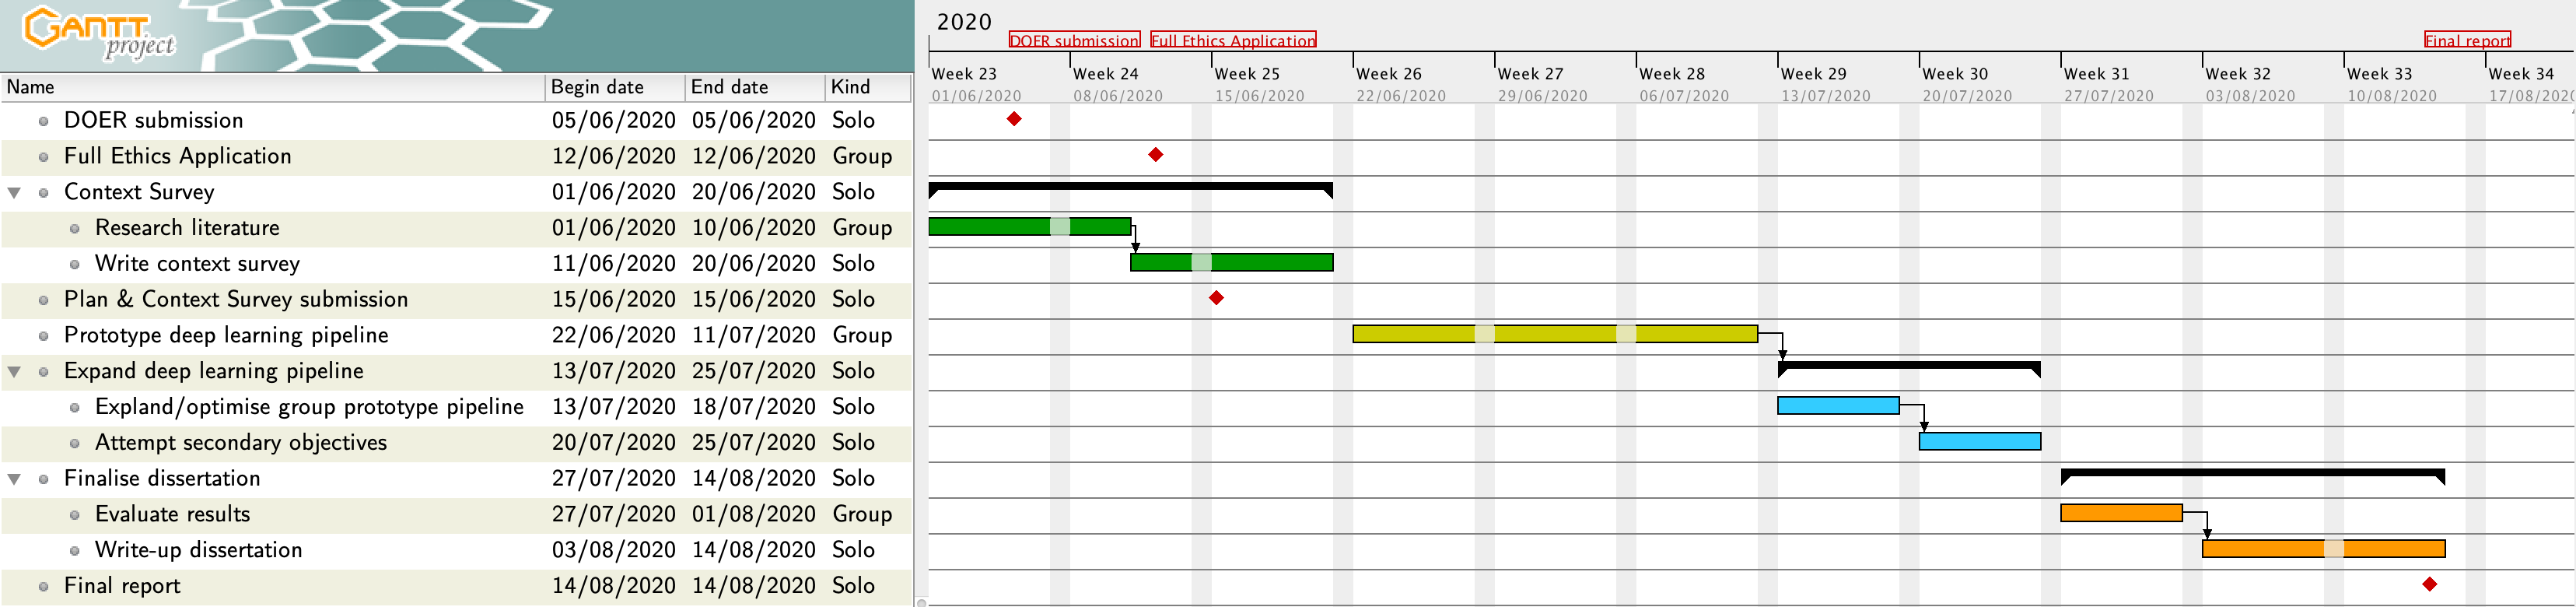
\includegraphics[width=\textwidth]{figures/gantt_chart.png}}
\caption{\label{fig:gantt_chart}Gantt Chart ranging from 01/06/2020 to 14/08/2020.}
\end{figure}


% ------------------- Draft Context Survey --------------------

\section{Draft Context Survey}
\label{sec:draft-context-survey}

\textit{\underline{Note}: According to the dissertation time plan expressed in Section~\ref{sec:time-plan}, the context survey will be finished by the end of week 3 (19/06/2020). Consequently, this context survey is still in a draft format. The majority of time has been invested in researching and taking notes on state-of-the-art papers (over 20 papers so far) and coming up with a detailed and logical plan. Sections with bullet points still need to be properly written while further information/references will be added to the existing parts.}

\subsection{Breast Cancer Detection}

\subsubsection{Early Breast Cancer Detection Systems}

% todo: explain what are mammograms -> support for why it's hard for radiologists alone to make decisions based on mammograms
% limitations of radiologists

The detection of breast cancer using mammograms, and any form of cancer using medical imagery, relies on the conventional diagnoses of expert radiologists \cite{Osareh2010}. These diagnoses rest on the correct interpretation of the mammograms, which may be subject to errors due to the difficulty of correctly interpreting them \cite{Elter2009}. Indeed, mammograms are 2D images of 3D breasts that correspond to the superposition of breast tissue, which increases the difficulty for a radiologist to correctly analyse patterns as masses often naturally form due to this superposition \cite{Elter2009}.\\

To assist radiologists in their interpretations of mammograms, Computer-Assisted Detection/Diagnosis (CAD) software have been employed since the 1970s. However, pre-1990s CAD systems were very primitive and did not offer much more knowledge than the expert radiologists'. These unsophisticated ``expert'' systems consisted of manually processing and modelling pixels to construct rule-based systems that mainly used \textit{if-else-then} statements \cite{Litjens2017}.

\subsubsection{Evolution towards Supervised Machine Learning-based Systems}

Supervised machine learning models have been applied to the problem of breast cancer detection since XXXX. However, these models could not accurately operate on purely raw data such as the full-sized mammogram images. Indeed, of the many machine learning models tested against the task of breast cancer detection such as k-Nearest Neighbour (kNN), Support Vector Machines (SVM), Decision Trees (DT), Random Forests (RF), Naive Bayes (NB) and Multi-Layer Perceptrons (MLP), these all require relevant bits of information to be extracted first in order to solve the given task. These important pieces of information correspond to features, and need to be extracted by humans before being fed to the aforementioned models for training. These features can range from colours, edges and corners to shapes and textures.\\

The next logical step in the evolution of breast cancer detection systems is for the selected model to learn these features on its own directly from the data rather than being fed hand-extracted features \cite{Yala2019}. Deep learning models, which corresponds to neural networks with hundreds of hidden layers, are based on this concept. However, these models have not been successfully implemented until recent years as they require powerful computers (usually equipped with Graphical Processing Units) to be efficiently trained. 

% History of breast cancer detection (leads to)\\
% Motivation of using ML/DL for breast detection\\
% Problems with current breast cancer detection systems

% ---------------

\subsection{Machine Learning models and breast cancer detection applications}

\subsubsection{Machine Learning tasks}

\textbf{Supervised \& unsupervised learning algorithms}\\

Machine learning algorithms come in many flavours, ranging from supervised and unsupervised learning to reinforcement learning. The two main types correspond to supervised and unsupervised learning \cite{Geron2019}. In supervised learning, a label $y$ is predicted based on input features $x$ by using a training dataset where the labels are known. During supervised training, the models' optimal parameters are determined to best predict the label.\\

On the other hand in unsupervised learning, the data is unlabelled, requiring the machine learning model to find patterns in the data by using known methods such as clustering and Principal Component Analysis (PCA) \cite{Litjens2017}.

\begin{itemize}
    \item Different types of learning model: supervised VS unsupervised (briefly mention semi-supervised and reinforcement learning). \textit{In this thesis, supervised learning used with labelled mammograms.}
\end{itemize}

\paragraph{Machine learning tasks applied to medical imagery analysis}

\begin{itemize}
    \item Classification
    \item Detection
    \item Segmentation
    \item Out-of-scope Machine Learning tasks in medical imagery analysis: registration, CBIR, image generation, image enhancement.
\end{itemize}

\subsubsection{Machine Learning models}

\begin{itemize}
    \item k-Nearest Neighbours
    \item Naive Bayes
    \item Support Vector Machines
    \item Decision Trees
    \item Random Forest
    \item Artificial Neural Networks
    \begin{itemize}
        \item Multi-Layer Perceptrons (shallow artificial neural networks)
        \item Deep neural networks
    \end{itemize}
\end{itemize}

For each, mention pros and cons based on existing papers and compare different approaches. Naturally lead towards deep neural networks (e.g. CNNs) for the final section.

% ---------------

\subsection{Deep Learning techniques \& Convolutional Neural Networks}

\subsubsection{Convolution Neural Networks}

\begin{itemize}
    \item Deep Neural Networks
    \item Convolutional Neural Networks
\end{itemize}

Explore the techniques used in deep learning (techniques, databases, processing, libraries, output metrics, etc.)\\
Explore the deep learning model that will be explored by each dissertation

\subsubsection{Rise of Deep Learning in Medical Imagery Analysis}

\begin{itemize}
    \item Evolution of CNNs (first CNN used, first CNN applied to medical imagery analysis, famous architectures e.g. LeNet, AlexNet, GoogLeNet, ResNet, etc.)
    \item Hardware advances (GPUs)
    \item Software advanced (libraries)
\end{itemize}


% -------------------- APPENDIX --------------------

\begin{appendices}

\clearpage
\bibliographystyle{unsrt}
\bibliography{bibliography}

\end{appendices}
\end{document}